\subsection{UCP}
\label{sec:algorithms:ucp}

Utility Cache Partition~\cite{Qureshi2006} (UCP) was first presented in 2006. 
UCP uses the concept of utility when assigning ways to a core.
Using a utility monitor (UMON), UCP divides the ways in the cache between the cores.
UCP then uses the same insertion and promotion policy as LRU.
The replacement policy is as in LRU but with two modifications:
First if the number of blocks owned by the requesting core is less than the number of ways assigned to it, then the least recently used block that is not assigned to the requester core is replaced.
If however the number of blocks owned is greater than or equal to the number of assigned ways the replacement algorithm selects the least recently used block of those owned by the requester.
This replacement policy ensures that the division between cores in each set move toward the global allocation following cache misses.
At the same time, a core may use more blocks that it is currently assigned, given that the space is not clamed by any other core.

The UMON is the core of the UCP algorithm.
It consists of one ATD per core sharing the cache. 
The ATD is managed by normal LRU replacement and has one access counter per way.
Whenever a cache request hits in the ATD, the access counter representing the way the block was in is incremented.
In other words, UMON uses the stack property of LRU, as explained in section~\ref{sec:algorithms:lru}, to find the hit rate of all valid partition sizes.
In addition to the ATDs, there is a monitor circuit that uses the access counters to caclulate a new global partition at set intervals.
In the original paper, the authors recalculate the partitioning every 5M cycles.

The original paper proposes several algorithms for determining optimal partitioning based on the counter data. 
On of them is a Lookahead Algorithm suitable when there are more than two cores sharing a cache.
The Lookahead Algorithm assigns ways based on an increase in marginal utility; it is given in Algorithm~\ref{alg:algorithms:ucp}.
While there are more ways to distribute, the algorithm calculates the maximum marginal utility achievable by each core. 
The core with the highest value wins and is assigned as many ways as needed to achieve the increase.
The algorithm continue until all ways have been assigned.
Lines 27-28 calculate the marginal utility. 
First the number of misses prevented by increasing the allocation from a to b is found.
Due to the stack property of LRU, this is simply done by summing the access counters for ways $a$ to $b-1$.
The number of misses is then divided by the number of sets introduced, to find the marginal utility.
The rest of the algorithm is simply a greedy algorithm selecting the highest marginal utility at each iteration.
After a reallocation of cache ways, the ATD counters are all halved.
By doing this, the UMON will keep historical data for future decisions while prioritizing data from the current period.

\begin{figure}[ht]
    \centering
    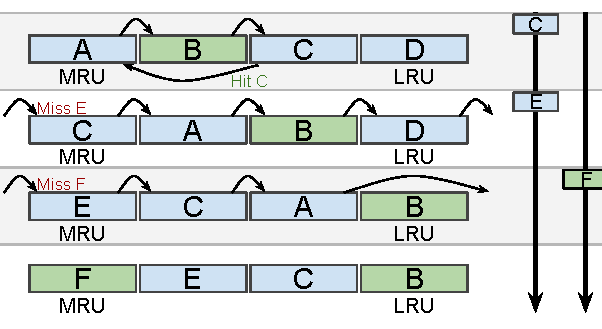
\includegraphics[width=.65\textwidth]{figures/algorithms/UCP}
    \caption[UCP managed 4-way cache set.]{UCP managed 4-way cache set. (Two cores each allocated two blocks)}
    \label{fig:algorithms:ucp_example}
\end{figure}

\begin{algorithm}[ht]
\caption{UMON Lookahead Algorithm.}
\label{alg:algorithms:ucp}
\begin{algorithmic}[1]
\State $balance\gets N$ /* Number of ways */
\State $allocations[i]\gets 0$  /* for each core $i$ */
\While {$balance$}
    \ForAll {$cores\ i$}
        \State $alloc\gets allocatations[i]$
        \State $max\_mu[i]\gets \Call{get\_max\_mu}{i, alloc, balance}$
        \State $blocks\_req[i]\gets$ min blocks to get max\_mu[i] for i
    \EndFor
    \State $winner\gets$ application with the maximum value of max\_mu
    \State $allocations[winner] += blocks\_req[winner]$
    \State $balance -= blocks\_req[winner]$
\EndWhile
\State \Return alloactions
\State

\Function{get\_max\_mu}{$i, alloc, balance$}
    \State $max\_mu\gets 0$
    \For{$ii = 1; ii <= balance; ii++$}
        \State $mu\gets \Call{get\_mu\_value}{p, alloc, alloc+ii}$
        \If{$mu \ge max\_mu$}
            \State $max\_mu\gets mu$
        \EndIf
    \EndFor
    \State \Return{$max\_mu$}
\EndFunction
\State

\Function{get\_mu\_value}{$p, a, b$}
    \State $U\gets$ change in misses for application p when number of blocks assigned to it increases from a to b
    \State \Return{$\frac{U}{b-a}$}
\EndFunction
\end{algorithmic}
\end{algorithm}


\todo{Example here}